\chapter{Web Tier}

\section{Java EE Architektur}

In Java EE gibt es die folgenden Architekturen:

\begin{description}
	\item[Web zentrische Architektur] Client greift nur auf einen Web Container zu, welche alle benötigten Komponenten beinhaltet.
	\item[B2B Architektur] Verwendet zwei EJB Server mit je einem Web- und EJB-Container.
	\item[Web Service Architektur] Eine Business-Komponente veröffentlicht Funktionalität über Web Service. Stateless Session Bean dient als Zugriffspunkt für die Servicefunktion.
\end{description}

Ausserdem erlaubt Java EE eine komponentenbasierte Entwicklung. Jede Komponente wird vom Container verwaltet, was die lokale und verteilte Interaktion unter den Komponenten erleichtert. Die Komponenten können durch einen Namensservice referenziert werden, was Standort-Transparenz ermöglicht. Die meisten Komponenten sind durch Interfaces definiert. Die Komponenten kommunizieren nur über das Interface miteinander (auch wenn auf gleicher JVM). Die Komponenten Infrastruktur stellt dafür auch Proxies zur Verfügung. Es gibt auch eine RMI Infrastruktur für verteilte Komponenten. Diese kümmert sich um das Marshalling/Unmarshalling von Argumenten und Rückgabewerten, das Übergeben von verteilten Exceptions und das Übergeben von Security- und Transaktions-Kontext.

\section{Servlet}

Ein Servlet ist ein Java Programm welches in einem Web- oder Applikationsserver läuft und das \verb|javax.servlet.Servlet|-Interface implementiert. Servlets werden für Anfragen und Antworten vom Internet Clients oder Browsers verwendet. Das Standard Protokoll für die Kommunikation zwischen Browser und Servlet ist HTTP oder HTTPS. Alle Servlets müssen das Servlet Interface direkt oder indirekt implementieren. Dazu schreiben Sie ein generisches Servlet das
\verb|javax.servlet.GenericServlet| erweitert oder ein HTTP-Servlet das \verb|javax.servlet.http.HttpServlet| erweitert.

Folgende Gründe sprechen für Servlets:

\begin{itemize}
	\item Verwaltet Anfragen und Antworten
	\item Multi Threading
	\item Verteilbar (RMI, Corba, INDI)
	\item Ein Heer von Programmierern
	\item Viele Komponenten verfügbar
	\item Sehr stabile Container (Tomcat, Jeronimo, Jetty)
	\item Ideal für kleine Applikationen (Servlets only)
\end{itemize}

Ein Nachteil von Servlets ist die langsame Entwicklung mit Servlets, weil die Applikation bei jeder Änderung neu kompiliert und deployt werden muss. Zudem ist HTML-Wissen (oder HTTP?) notwendig. Abbildung \ref{fig:servlet-aufruf} zeigt eine Beispiel-Anfrage an ein Servlet. Der Server identifiziert das Servlet gemäss der URL (web.xml) und delegiert die Anfrage zum Servlet. Danach führt das Servlet seine Arbeit (z.B. EJB-Aufruf) aus und produziert eine Antwort (formatierte HTML-Seite). Der Server sendet die Antwort zum Client zurück.

\begin{figure}
\centering
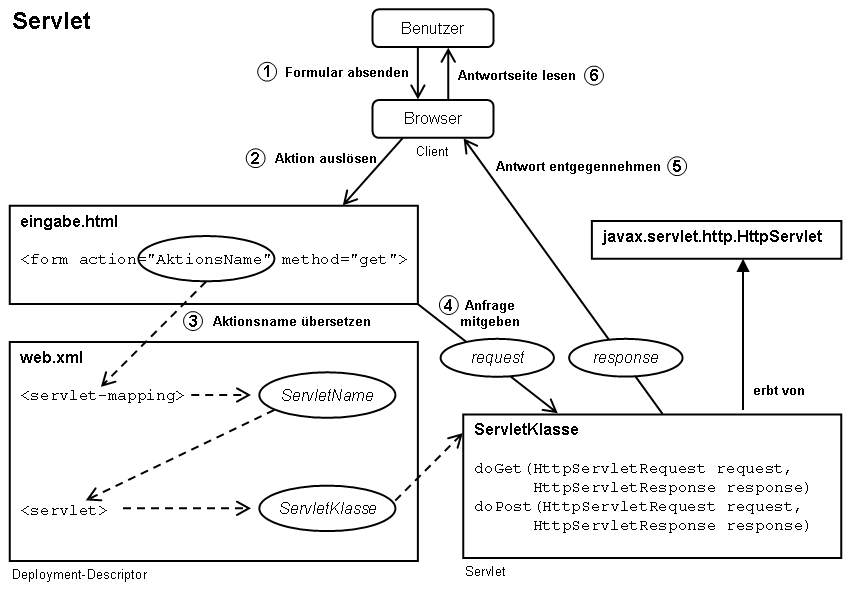
\includegraphics[width=0.7\linewidth]{fig/servlet-aufruf}
\caption{Servlet Aufruf}
\label{fig:servlet-aufruf}
\end{figure}

\subsection{Life Cycle}

Abbildung \ref{fig:servlet-life-cycle} zeigt den Life Cycle eines Servlets. Die Methoden \verb|init()| bzw. \verb|destroy()| werden jeweils beim Applikationsstart/-ende aufgerufen. Bei jedem Request wird die \verb|service()|-Methode aufgerufen. Diese kümmert sich um die Weiterleitung an die entsprechenden HTTP-Methoden (\verb|doGet()|, \verb|doPost()|, \verb|doPut()| usw.), welche der Entwickler implementiert.

\begin{figure}
\centering
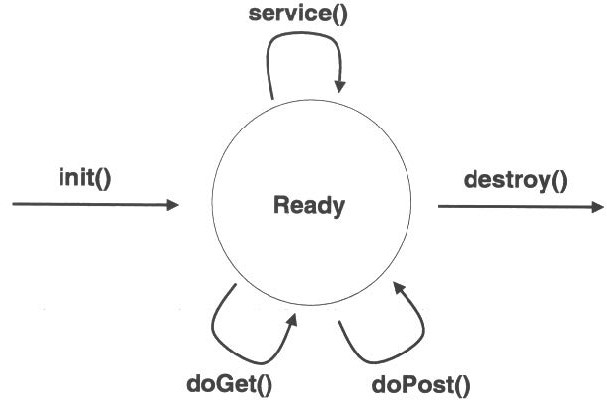
\includegraphics[width=0.5\linewidth]{fig/servlet-life-cycle}
\caption{Servlet Life Cycle}
\label{fig:servlet-life-cycle}
\end{figure}

\subsection{Nebenläufigkeit}

Im Gegensatz zum EJB-Container ist man im Servlet-Container selbst verantwortlich für die Nebenläufigkeit. Wenn mehrere Anfragen gleichzeitig an das Servlet gestellt werden, greifen mehrere Threads gleichzeitig auf z.B. Instanzvariablen eines Servlets zu. Deshalb sollte der Entwickler folgende Punkte beachten:

\begin{itemize}
	\item Instanzvariablen mit Vorsicht verwenden (Besser lokale oder finale Variablen)
	\item Klassenvariablen mit Vorsicht verwenden
	\item Den Zugriff auf externe Ressourcen vorsichtig abwickeln (DB ist selten das Problem - eher Zugriff auf Filesystem)
	\item Synchronisationsprimitiven für kritische Abschnitte benutzen
\end{itemize}

\subsection{Session Management}

Das Session Management kann im Web Tier über Session Cookies oder über eine Session ID realisiert werden. Man sollte die Session ID verwenden, weil diese vom Container verwaltet wird und nur die ID im Cookie gespeichert (Es ist auch möglich ID an URL anzuhängen aber lass das bitte sein) wird. Der Entwickler braucht sich nicht mehr um das Session-Management kümmern.

\subsection{Scopes}

Eine Bean muss einen gewissen Zustand halten während ein Anwender mit der Applikation interagiert. Der Zustand wird über Scopes definiert. Es gibt folgende Scopes, welche mit Annotations markiert werden können:
\begin{description}
	\item[Application] gültig über alle User-Aktionen mit der Applikation . Alle JSP oder Servlets können auf diese Beans zugreifen (z.B. Datenbankzugriff).
	\item[Session] gültig über mehrere HTTP Anfragen. Ein Bean wird erzeugt und mit der aktuellen Session verknüpft. Nachfolgende Anfragen vom selben Benutzer haben Zugriff darauf (z.B. Warenkorb).
	\item[Flow] gültig während eines spezifischen Ablaufs mit der Applikation (neu in Java EE 7). 
	\item[Request] Gültig während einer einzigen HTTP Anfrage. Bean wird erzeugt und im aktuellen Request-Objekt abgelegt (z.B. Suche).
	\item[Dependent] Kennzeichnet eine Abhängigkeit von einem anderen Bean.
\end{description}

\subsection{Filter}

Mit Filtern kann eine Anfrage vor dem Verarbeiten durch ein Servlet ausgelesen und evtl. verändert werden (z.B. Logging aller Anfragen). Filter lassen sich verketten und verschachteln. Ein Filter ist eine simple Java Klasse die das \verb|javax.servlet.Filter|-Interface implementiert. Wichtig ist die \verb|doFilter((ServletRequest, ServletResponse, FilterChain))|-Methode. Danach kann man den Filter mit der \verb|@WebFilter|-Annotation oder im web.xml registrieren.

\section{Java Server Faces}

Die aktuelle View-Technologie sind die Java Server Faces (JSF). JSF basiert wiederum auf den Java Server Pages (JSP), welche heute aber nicht mehr verwendet werden. Eine JSP muss bei ihrem ersten Aufruf zuerst kompiliert werden, was eine gewisse Zeit dauert. Ist sie aber einmal kompiliert, wird sie im Memory gecached und kann schneller ausgeliefert werden. Mit JSP kann man Templates schreiben die HTML, CSS und Javascript benutzen. Es kann aber auch direkt Java-Code verwendet werden (\verb|<% // Java Code %>|). Zudem gibt es \textit{taglibs} welche auf Java Code zeigen und so den Programmfluss steuern.

Mit JSF wurde 2004 ein Komponenten basiertes Framework vorgestellt, welches einen verbesserten MVC Ansatz und Ajax Unterstützung mitbringt. Listing \ref{lst:jsf-beispiel} zeigt ein simples JSF Beispiel.

\begin{lstlisting}[caption=JSF Beispiel, label=lst:jsf-beispiel]
// Bean erstellen (HelloWorld.java)
@ManagedBean(name = "HelloWorld", eager = true)
public class HelloWorld {

	public String getMessage() {
		return "Hello World!";
	}
}

// Faces Servlet konfigurieren (web.xml)
<welcome-file-list>
	<welcome-file>faces/home.xhtml</welcome-file>
</welcome-file-list>

// JSF Page erstellen (home.xhtml)
<head>
	<title>JSF Beispiel!</title>
</head>
<body>
	#{helloWorld.message}
</body>
\end{lstlisting}

JSF bringt diverse Taglibraries mit um HTML und Java zu verknüpfen. Die \textit{html basic} Taglibrary (\verb|h:|) definiert Tags für gängige HTML Komponenten. Die jsf core Taglibrary (\verb|f:|) definiert alle anderen Tags der JSF. Es handelt sich dabei um XML-Namensräume, welche nicht verschachtelt werden sollten.

\section{Java EE Patterns}
Java EE Patterns sind Muster/Best Practices, wie konkrete Probleme im Java EE Umfeld elegant gelöst werden können. Die Muster sind nicht teil der Prüfung und evtl. sollte man sich Gedanken machen welches Muster man in seiner Applikation verwendet hat.

\subsection{Model View Controller (MVC)}

Im klassischen MVC-Pattern (siehe Abbildung \ref{fig:mvc1}) wird die View über Events informiert, wenn sich das Model geändert hat. Dieses Verhalten ist aber nicht optimal für Webanwendungen, weil geänderte Daten nur bei einem Request gezeigt werden müssen. Deshalb wurde das MVC-Pattern leicht abgeändert (siehe Abbildung \ref{fig:mvc2}). Der Controller ist ein Servlet, welches den Request ausliest, die View aussucht und die entsprechenden Daten dem Model übergibt. Der Entwickler merkt vom Controller nichts, weil der bereits implementiert wurde. Das Model ist eine Java Bean (.java), welche auf das Business-Layer zugreifen kann. Die View holt sich dann die Daten vom Model und ersetzt sie im Template (.xhtml). Dann wird der View mit den eingesetzten Daten zurückgesendet.

\begin{figure}
	\centering
	\begin{subfigure}[b]{0.5\textwidth}
		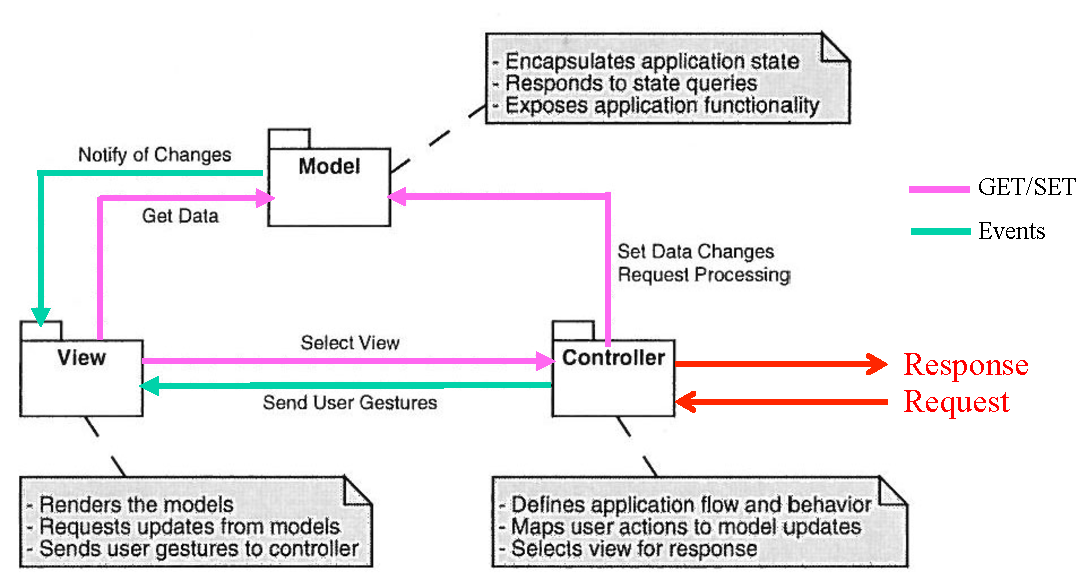
\includegraphics[width=\textwidth]{fig/mvc1}
		\caption{Ursprüngliches MVC}
		\label{fig:mvc1}
	\end{subfigure}
	~
	\begin{subfigure}[b]{0.4\textwidth}
		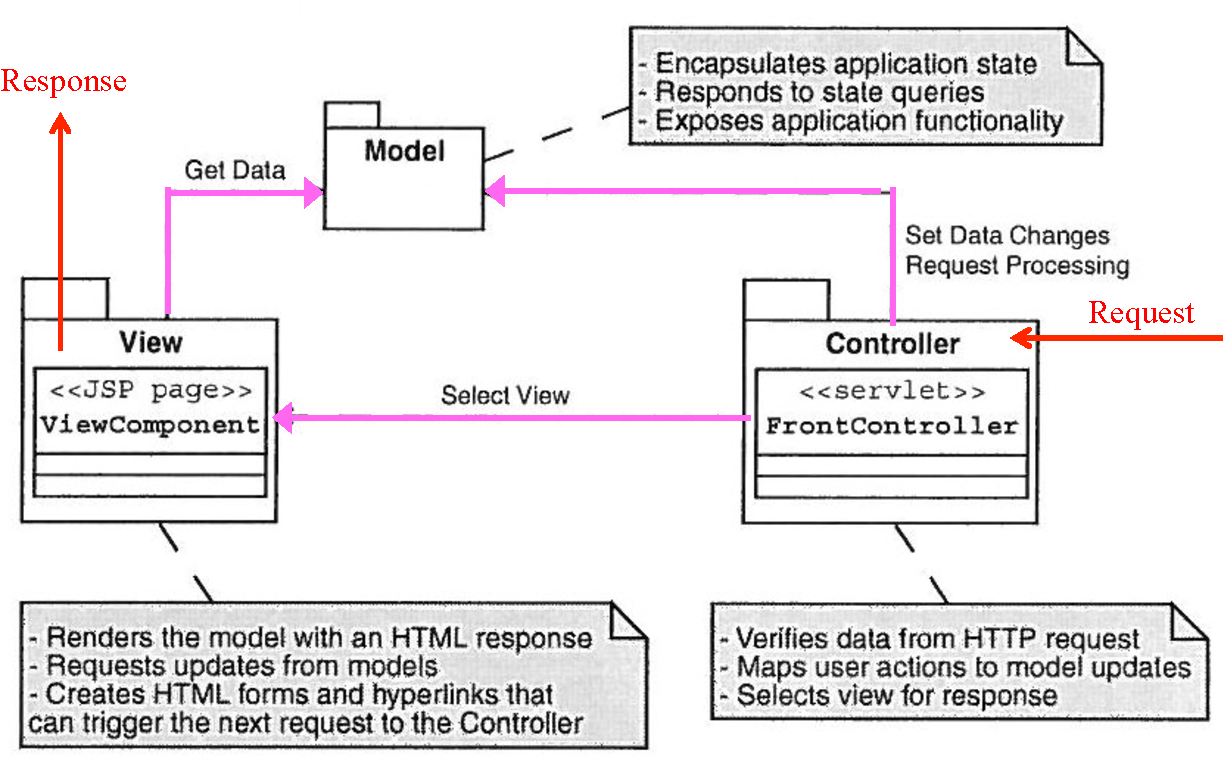
\includegraphics[width=\textwidth]{fig/mvc2}
		\caption{MVC für Web}
		\label{fig:mvc2}
	\end{subfigure}
	\caption{Model View Controller}
\end{figure}

\subsection{Service Locator}

Der Service Locator ist eine globale Anlaufstelle um einen Service zu beziehen. Dadurch wird der Service von der konkreten Implementation entkoppelt. Dadurch lassen sich Implementationen zur Laufzeit austauschen (z.B. bessere JPG-Komprimierung verfügbar - Austausch ohne Neustart). Weil es nur einen Service Locator gibt kann dieser schnell zum Flaschenhals werden. Zudem werden die Abhängigkeiten im System verschleiert.

\subsection{View Helper}

Da sich die View häufig ändert und die Business Logik relativ stabil bleibt, möchte man diese beiden Teile mehr voneinander entkoppeln. Ein View Helper ist eigentlich ein Adapter zwischen der Business Logik und dem View.

\subsection{Session Facade}

Mit einer Session Facade können Business Funktionen anderen Clients angeboten werden. Dabei wird die feinkörnige Businesslogik meist zu einer groben Funktion zusammengefasst.

\subsection{Data Access Object}

Der Zugriff und die Manipulation der Daten soll in einem separaten Layer gekapselt werden. 